\chapter{Supplementary results}
This chapter includes the supplementary results mentioned in the thesis but are the central part of discussions.

\section{Fundamental analysis of PAH growth models}
\subsection{Methane pyrolysis in shock tube}
\begin{figure}[H]
	\centering
	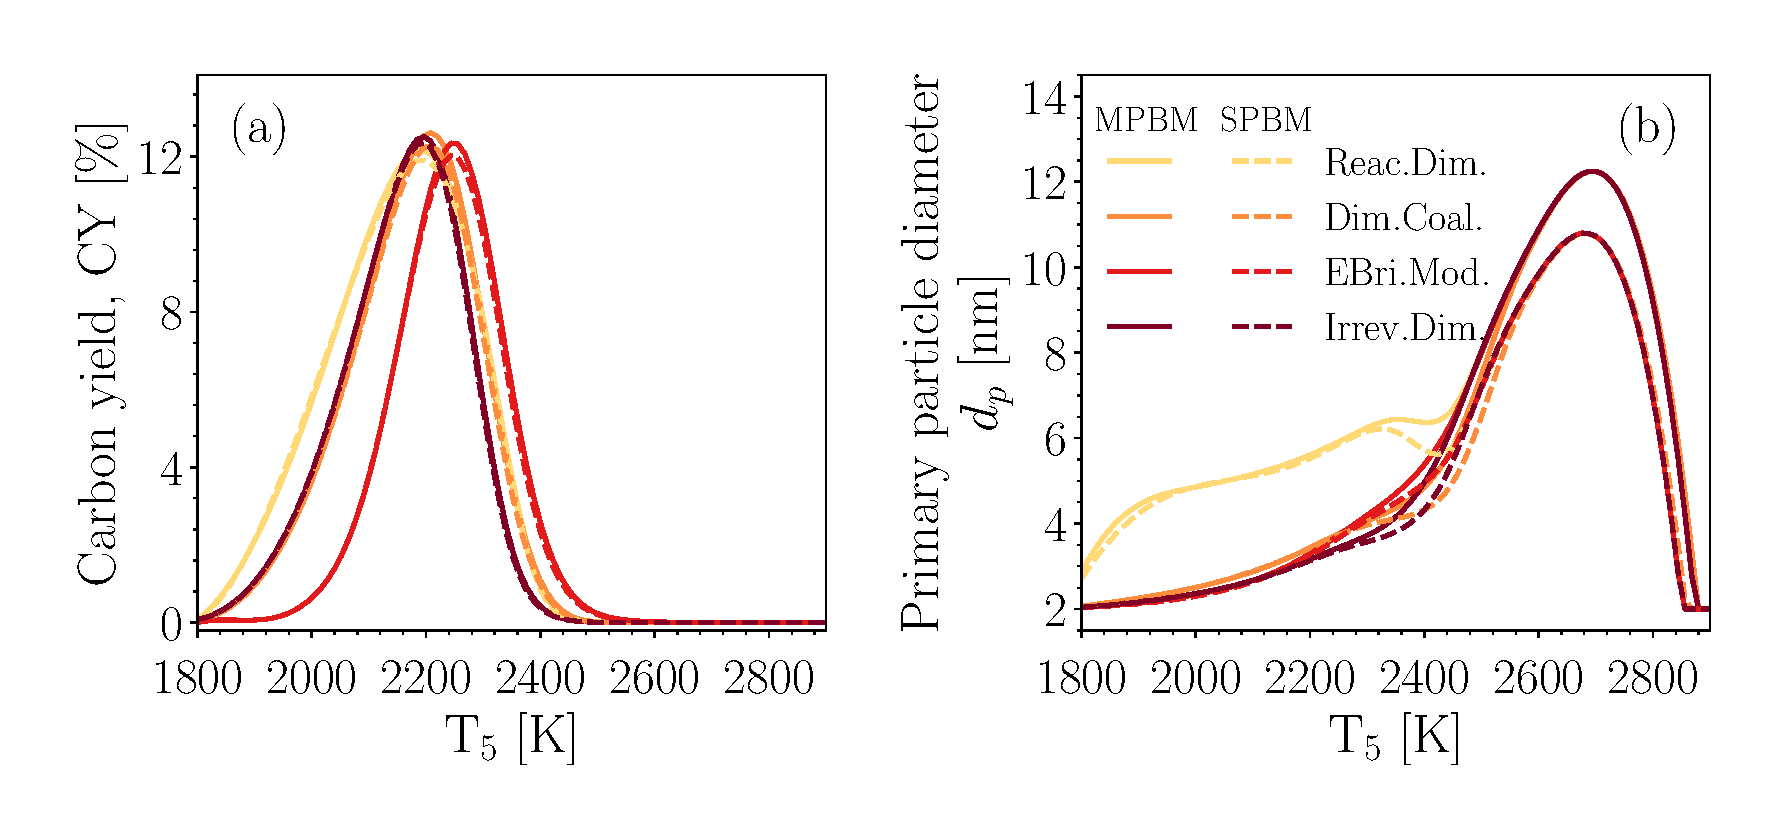
\includegraphics[width=0.8\textwidth]{Figures/Results/Paper1/Shocktube/Agafonov2016_cpr/carbon_yield_d_p_pdynamics.pdf};
	\caption{The comparison of CY (a) and primary particle diameter, $d_p$, at $t=$1.5 ms obtained using MPBM and SPBM models for the case optimized using equal adjustment factors to minimize the prediction error.}
	\label{fig:shockagof_yield_dp_cpr_pdynamics} 
\end{figure}


\begin{figure}[H]
	\centering
	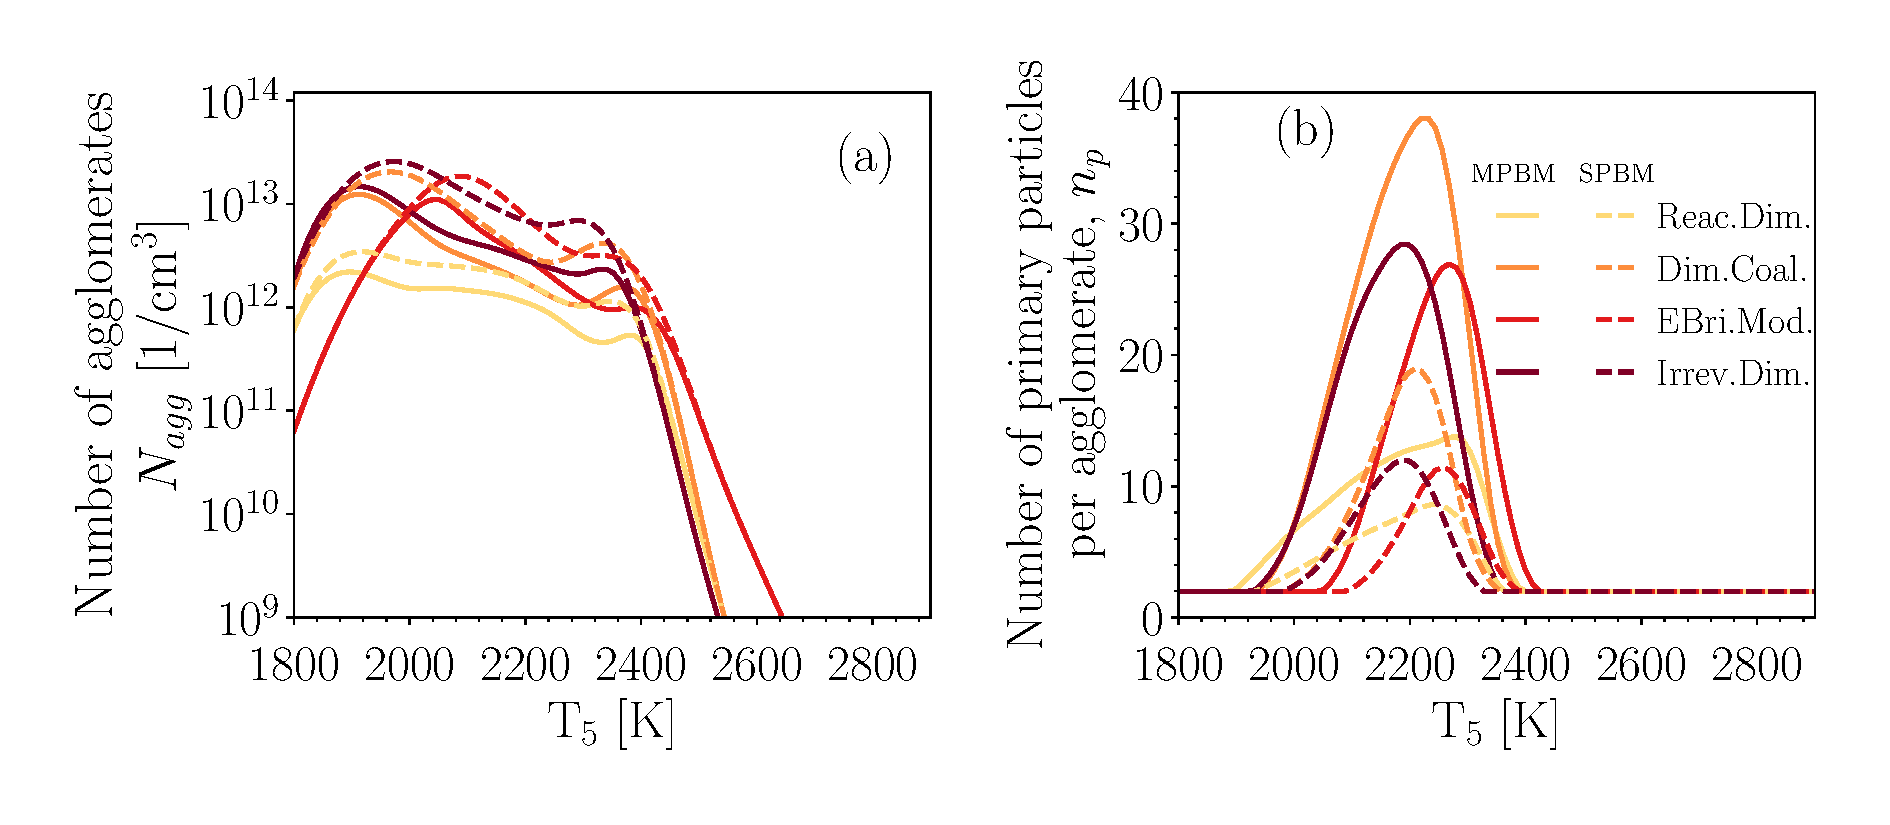
\includegraphics[width=0.8\textwidth]{Figures/Results/Paper1/Shocktube/Agafonov2016_cpr/N_agg_n_p_pdynamics.pdf};
	\caption{The temperature dependence of total number of agglomerates, $N_{agg}$ (a), number of primary particles per agglomerate, $n_p$ (b), at $t=$1.5 ms obtained using MPBM and SPBM models for the case optimized using equal adjustment factors to minimize the prediction error.}
	\label{fig:shockagof_N_agg_n_p_cpr_pdynamics} 
\end{figure}

\begin{figure}[H]
	\centering
	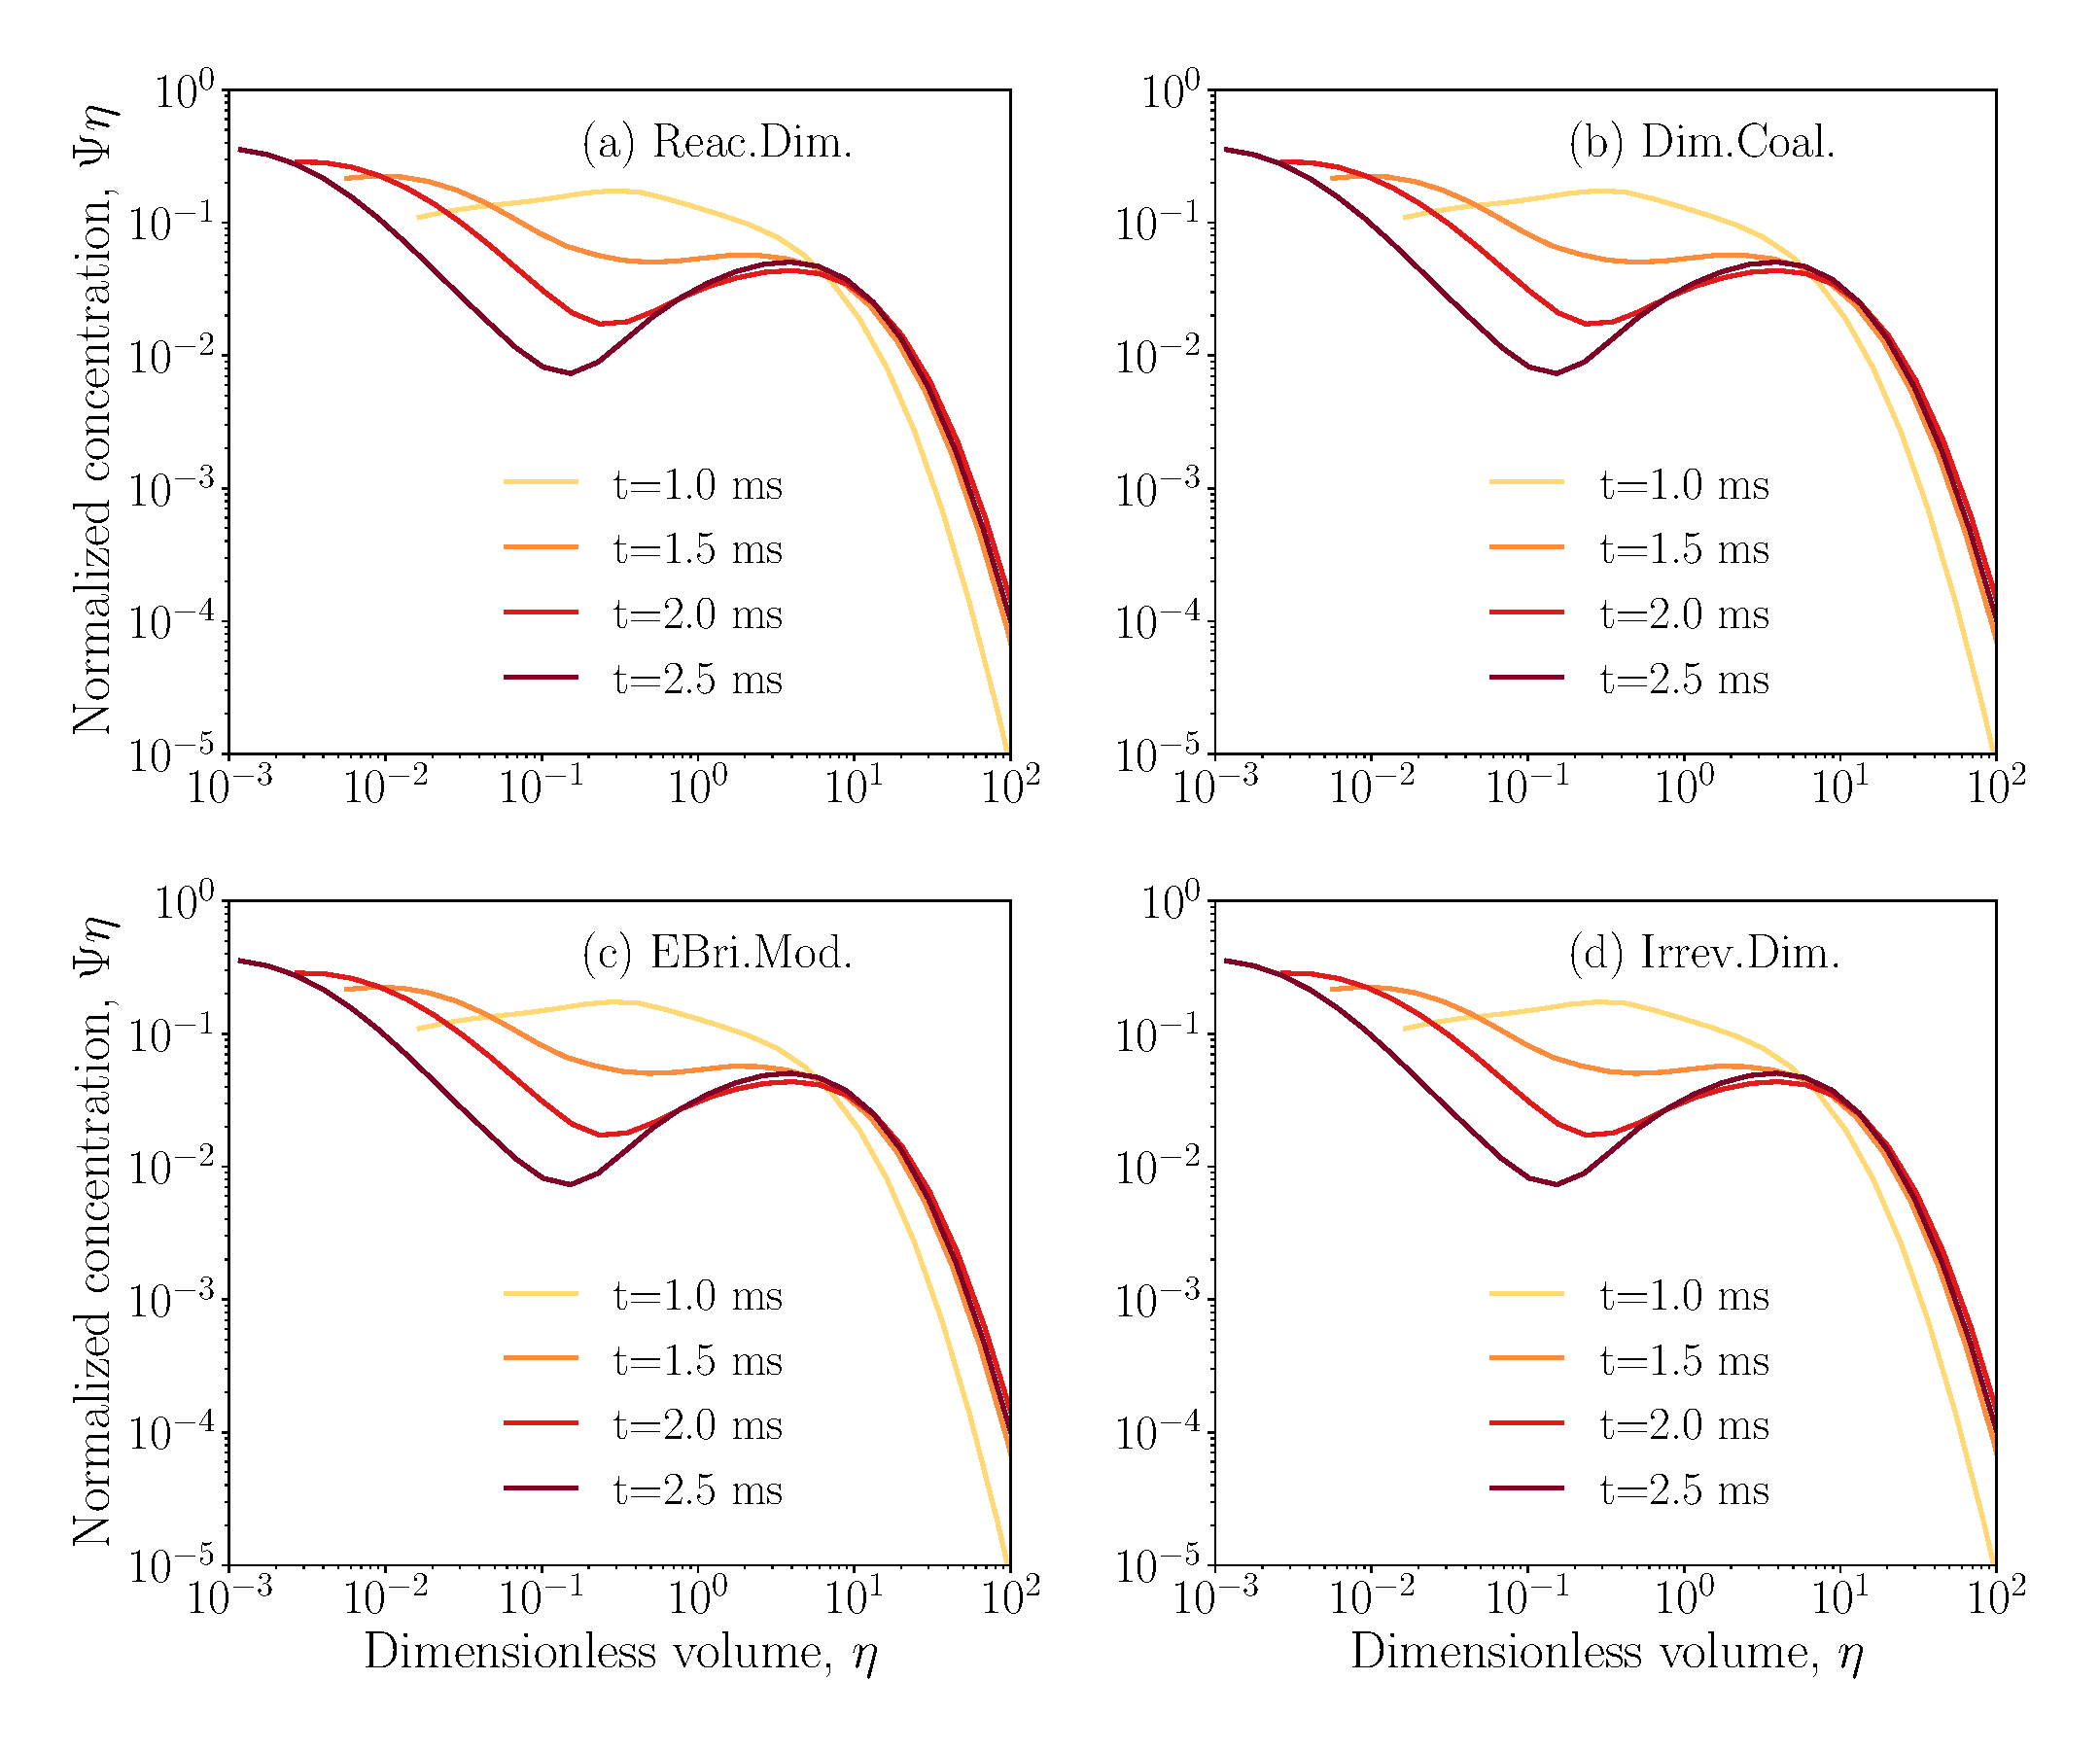
\includegraphics[width=0.8\textwidth]{Figures/Results/Paper1/Shocktube/Agafonov2016_cpr/5CH4_psd.pdf};
	\caption{The non-dimensional particle size distribution during 5\%$\mathrm{CH_4}$-Ar at $\mathrm{T_5}=2200$ K that evolves from 1~ms to 2.5~ms indicating SPSD is not attained yet.}
	\label{fig:shockagof_psd} 
\end{figure}

%------------------------------------------------------------------------------
%------------------------------------------------------------------------------
%------------------------------------------------------------------------------

\section{Ethylene pyrolysis in a flow reactor}



\begin{figure}[H]
	\centering
	\begin{tikzpicture}
		\draw (0, 0) node[inner sep=0] 	{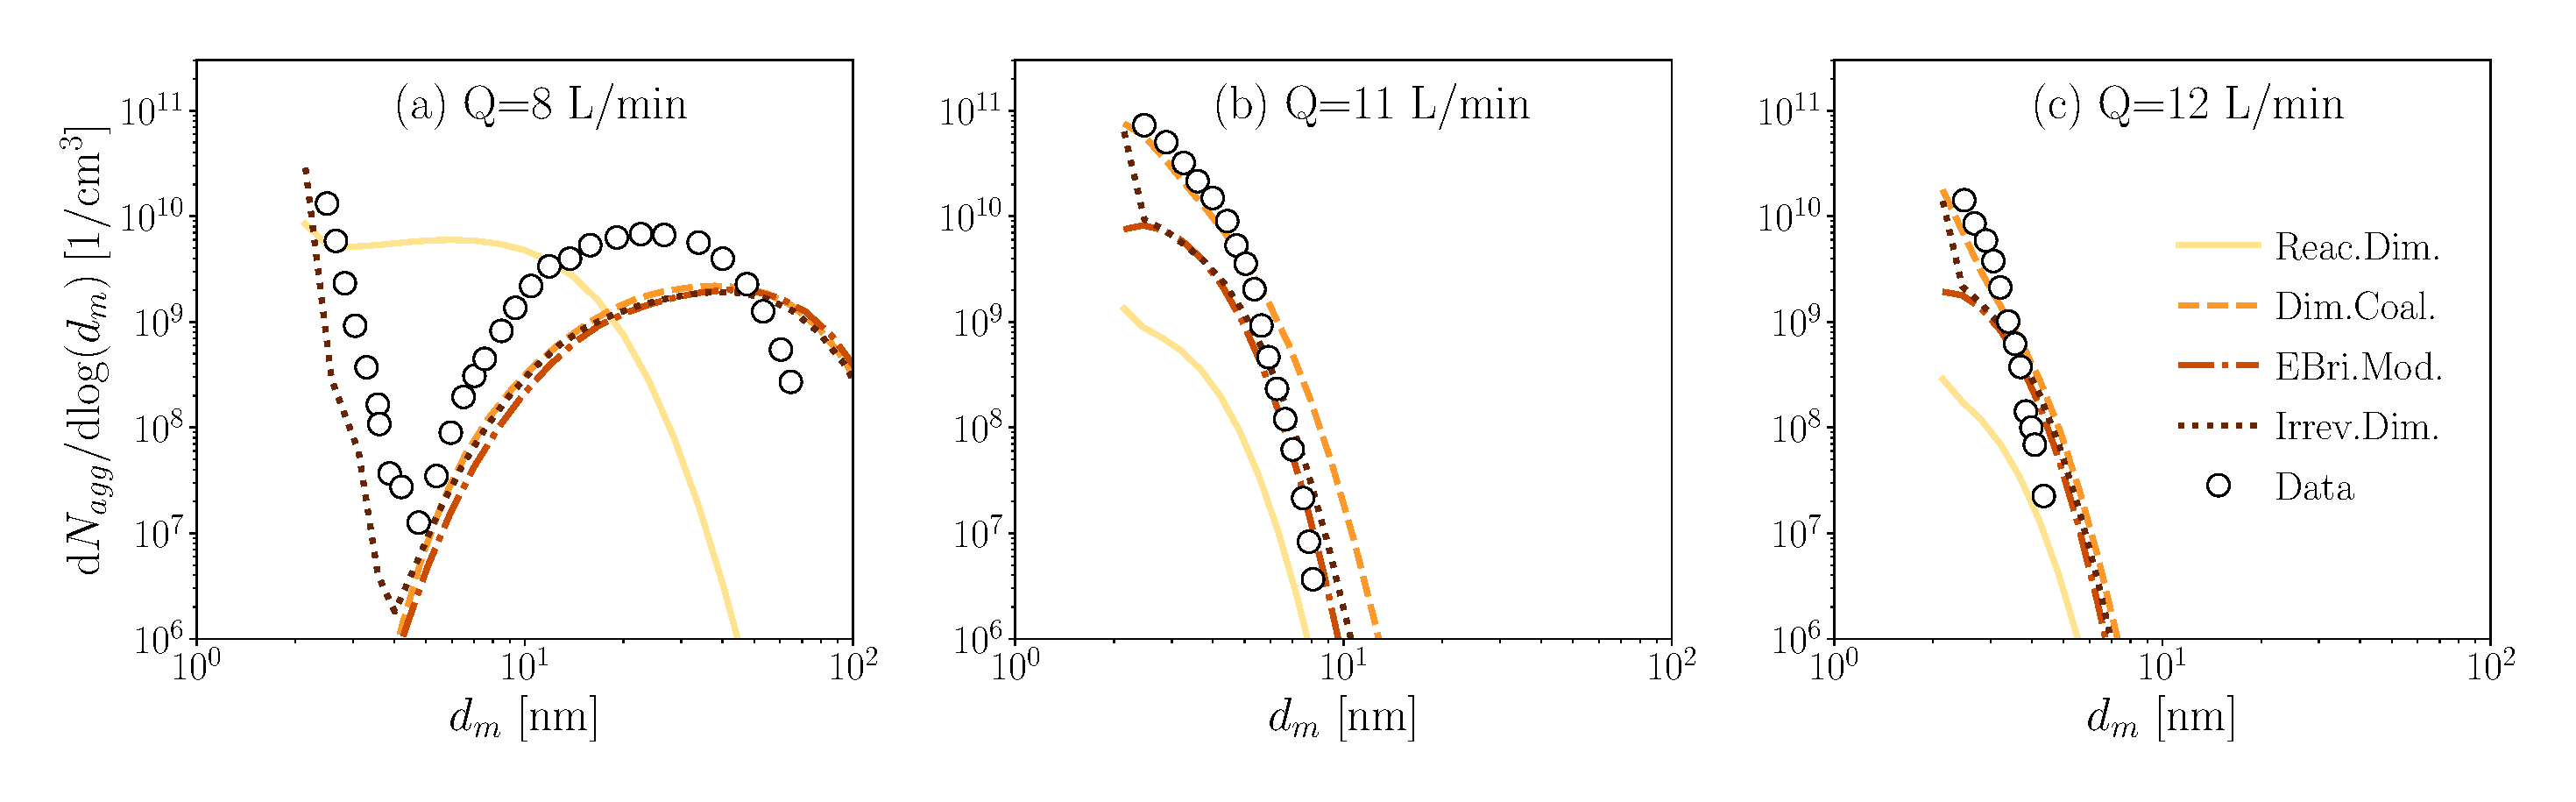
\includegraphics[width=1\textwidth]{Figures/Results/Paper1/PFR/PSD_diffQ_caltech.pdf}};
		\draw (7.1, -0.56) node {\scriptsize{\cite{mei2019quantitative}}};
	\end{tikzpicture}
	\caption{The particle size distribution at the end of PFR for $\mathrm{Q}=8$ (a), 11 (b), and 12 L/min (c) obtained using Caltech mechanism, SPBM and different inception models calibrated to match the predictions with measurement~\citep{mei2019quantitative}.}
	\label{fig:pfr_psd_caltech} 
\end{figure}


\begin{figure}[H]
	\centering
	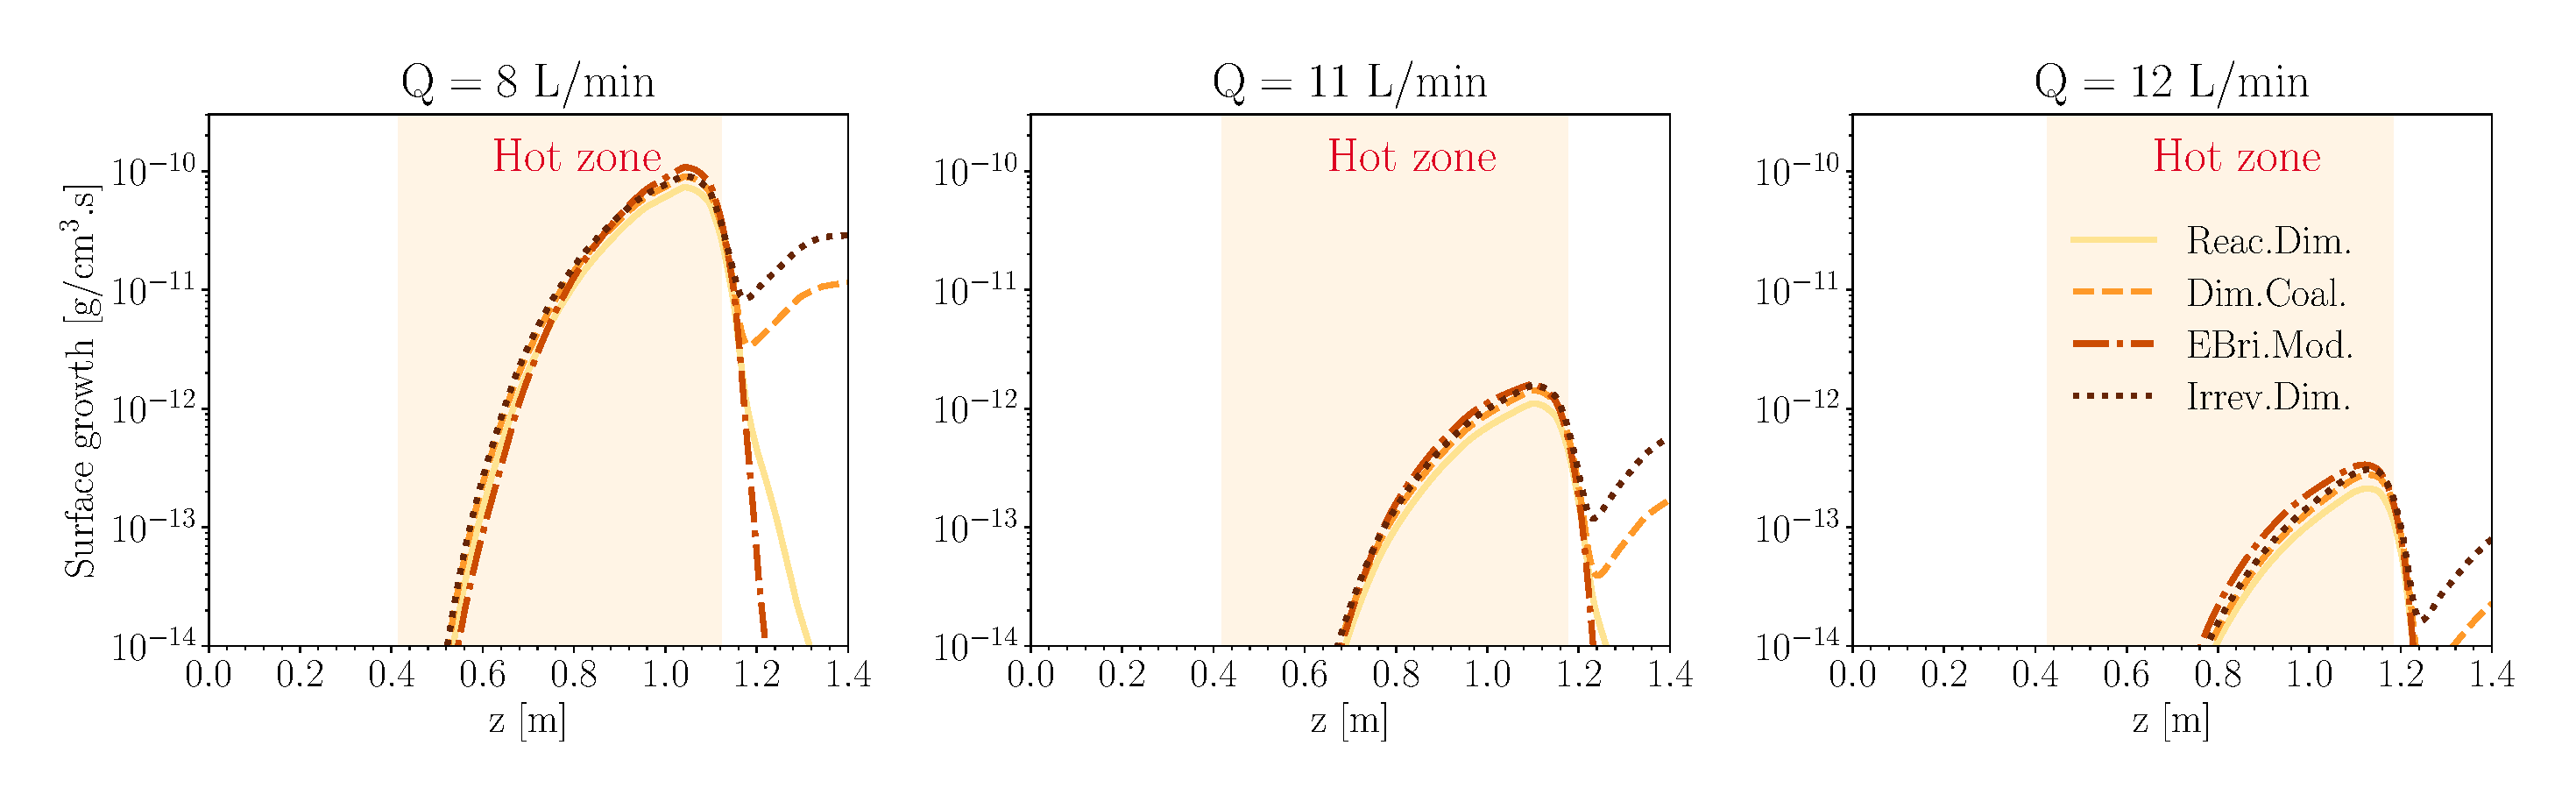
\includegraphics[width=1\textwidth]{Figures/Results/Paper1/PFR/surface_growth.pdf}
	\caption{The surface growth by HACA and PAH adsorption combined along the PFR for $\mathrm{Q}=8$ (a), 11 (b), and 12 L/min (c) obtained using KAUST mechanism, SPBM and different inception models. The yellow area represents the hot zone ($\mathrm{T}>0.9\mathrm{T_{max}}$).}
	\label{fig:pfr_surfacegrowth} 
\end{figure}
